\documentclass[12pt,a4paper,fleqn]{narms}

% packages needed
\usepackage{subfigure}
\usepackage{epsfig}
\usepackage{timesmt}

% add here more packages based on the document format

\usepackage[utf8]{inputenc}
\usepackage[OT1]{fontenc}
\usepackage{graphicx}
\usepackage[english]{babel}

\usepackage{amsmath}
\usepackage{amsfonts}
\usepackage{amssymb}
\usepackage{amsthm}
\usepackage{bm}

\usepackage[usenames,dvipsnames]{xcolor}
\usepackage{url}
\usepackage{tikz}
\usetikzlibrary{shapes.misc,fit}


\usepackage[bookmarks]{hyperref}

\usepackage{chicaco}

% setting math equation indent from left 0pts

%\mathindent=0pt%

\newcommand{\reals}{\mathbb{R}}
\newcommand{\posreals}{\reals_{>0}}
\newcommand{\posrealszero}{\reals_{\ge 0}}
\newcommand{\naturals}{\mathbb{N}}

\newcommand{\dd}{\,\mathrm{d}}

\newcommand{\mbf}[1]{\mathbf{#1}}
\newcommand{\bs}[1]{\boldsymbol{#1}}
\renewcommand{\vec}[1]{{\bm#1}}

\newcommand{\uz}{^{(0)}} % upper zero
\newcommand{\un}{^{(n)}} % upper n
\newcommand{\ui}{^{(i)}} % upper i

\newcommand{\ul}[1]{\underline{#1}}
\newcommand{\ol}[1]{\overline{#1}}

\newcommand{\Rsys}{R_\text{sys}}
\newcommand{\lRsys}{\ul{R}_\text{sys}}
\newcommand{\uRsys}{\ol{R}_\text{sys}}

\newcommand{\Fsys}{F_\text{sys}}
\newcommand{\lFsys}{\ul{F}_\text{sys}}
\newcommand{\uFsys}{\ol{F}_\text{sys}}

\def\Tsys{T_\text{sys}}

\newcommand{\E}{\operatorname{E}}
\newcommand{\V}{\operatorname{Var}}
\newcommand{\wei}{\operatorname{Wei}} % Weibull Distribution
\newcommand{\ig}{\operatorname{IG}}   % Inverse Gamma Distribution

\def\yz{y\uz}
\def\yn{y\un}
%\def\yi{y\ui}
\newcommand{\yfun}[1]{y^{({#1})}}
\newcommand{\yfunl}[1]{\ul{y}^{({#1})}}
\newcommand{\yfunu}[1]{\ol{y}^{({#1})}}

\def\ykz{y\uz_k}
\def\ykn{y\un_k}

\def\yzl{\ul{y}\uz}
\def\yzu{\ol{y}\uz}
\def\ynl{\ul{y}\un}
\def\ynu{\ol{y}\un}
\def\yil{\ul{y}\ui}
\def\yiu{\ol{y}\ui}

\def\ykzl{\ul{y}\uz_k}
\def\ykzu{\ol{y}\uz_k}
\def\yknl{\ul{y}\un_k}
\def\yknu{\ol{y}\un_k}


\def\nz{n\uz}
\def\nn{n\un}
%\def\ni{n\ui}
\newcommand{\nfun}[1]{n^{({#1})}}
\newcommand{\nfunl}[1]{\ul{n}^{({#1})}}
\newcommand{\nfunu}[1]{\ol{n}^{({#1})}}

\def\nkz{n\uz_k}
\def\nkn{n\un_k}
\newcommand{\nkzfun}[1]{n\uz_{#1}}


\def\nzl{\ul{n}\uz}
\def\nzu{\ol{n}\uz}
\def\nnl{\ul{n}\un}
\def\nnu{\ol{n}\un}
\def\nil{\ul{n}\ui}
\def\niu{\ol{n}\ui}

\def\nkzl{\ul{n}\uz_k}
\def\nkzu{\ol{n}\uz_k}
\def\nknl{\ul{n}\un_k}
\def\nknu{\ol{n}\un_k}


\def\taut{\tau(\vec{t})}
\def\ttau{\tilde{\tau}}
\def\ttaut{\ttau(\vec{t})}

\def\MZ{\mathcal{M}\uz}
\def\MN{\mathcal{M}\un}

\def\MkZ{\mathcal{M}\uz_k}
\def\MkN{\mathcal{M}\un_k}

\def\PkZ{\Pi\uz_k}
\def\PkN{\Pi\un_k}
\newcommand{\PZi}[1]{\Pi\uz_{#1}}


\def\tnow{t_\text{now}}
\def\tpnow{t^+_\text{now}}

\newcommand{\comments}[1]{{\small\color{gray} #1}}

\newtheorem{example}{Example}

\allowdisplaybreaks

\title{Notes for ISIPTA poster}
\author{Gero Walter, Frank P.A. Coolen, Simme Douwe Flapper}

\begin{document}
\maketitle

(Notation more similar to risk analysis paper.)

System with components of $k=1,\ldots,K$ different types.
There are $n_k$ components of type $k$ in the system.

For each $k$, component lifetimes ($i=1,\ldots,n_k$) are $T_i^k \mid \lambda_k \sim \wei(\kappa,\lambda_k)$,
where $\kappa$ is fixed and known:
\begin{align}
f_k(t_i^k \mid \lambda_k) &= \frac{\kappa}{\lambda_k} (t_i^k)^{\kappa-1} e^{-\frac{(t_i^k)^{\kappa-1}}{\lambda_k}} \\
F_k(t_i^k \mid \lambda_k) &= 1 - e^{-\frac{(t_i^k)^{\kappa-1}}{\lambda_k}} = P_k(T_i^k \leq t_i^k \mid \lambda_k)
\end{align}

Conjugate prior is $\lambda_k \sim \ig(\alpha_k,\beta_k)$:
\begin{align}
f_{\lambda_k}(\lambda_k\mid \alpha_k,\beta_k) &= \frac{(\beta_k)^{\alpha_k}}{\Gamma(\alpha_k)} \lambda_k^{-\alpha_k -1} e^{-\frac{\beta_k}{\lambda_k}}
\end{align}
In terms of canonical parameters $\nkz,\ykz$, $\lambda_k \mid \nkz,\ykz \sim \ig(\nkz + 1, \nkz\ykz)$.

Set of priors $\MkZ$ defined by $(\nkz,\ykz) \in \PkZ = [\nkzl,\nkzu] \times [\ykzl,\ykzu]$.

Observing a one of a kind system with $n_k$ components of type $k$ running until $\tnow$,
where $e_k$ components have failed by $\tnow$, and $n_k - e_k$ components still function:
\begin{align}
\mbf{t}^k_{e_k;n_k} &= \big( \underbrace{t^k_1, \ldots, t^k_{e_k}}_{e_k \text{failure times}},
                             \underbrace{\tpnow, \ldots, \tpnow}_{n_k-e_k \text{censored obs.}} \big)
\end{align}

Posterior:
\begin{align}
f_{\lambda_k\mid\ldots}(\lambda_k\mid\nkz,\ykz,\mbf{t}^k_{e_k;n_k})
 &\propto f_{\lambda_k}(\lambda_k)
          \big[ 1- F_k(\tnow\mid\lambda_k) \big]^{n_k-e_k}
          \prod_{i=1}^{e_k} f_k(t_i^k \mid \lambda_k) 
\end{align}
and so $\lambda_k\mid\nkz,\ykz,\mbf{t}^k_{e_k;n_k} \sim \ig(\nkn + 1, \nkn\ykn)$, where
\begin{align}
\nkn + 1 &= \nkz + e_k + 1 \\
\nkn\ykn &= \nkz\ykz + (n_k-e_k) \tnow^\kappa + \sum_{i=1}^{e_k} (t_i^k)^\kappa
\end{align}
so the posterior expectation for $\lambda$ is
\begin{align}
\E[\lambda_k\mid\nkn,\ykn] &= \ykn
                            = \frac{\nkz}{\nkz + e_k} \ykz +
                              \frac{e_k}{\nkz + e_k} \cdot \frac{1}{e_k}\Big[(n_k-e_k) \tnow^\kappa + \sum_{i=1}^{e_k} (t_i^k)^\kappa \Big]
\end{align}

%\newpage

System survival calculated by (see Risk Analysis paper eq. (7))
\begin{align}
P(\Tsys > t) &= \sum_{l_1=0}^{n_1} \cdots \sum_{l_K=0}^{n_K} \Phi(l_1,\ldots,\l_K) P\Big( \bigcap_{k=1}^K \{ C^k_t = l_k\} \Big) \\
\intertext{ and assuming components of different types are independent,}
             &= \sum_{l_1=0}^{n_1} \cdots \sum_{l_K=0}^{n_K} \Phi(l_1,\ldots,\l_K) \prod_{k=1}^K P(C^k_t = l_k)
\end{align}
where the survival signature $\Phi(l_1,\ldots,\l_K)$ is non-decreasing in each $l_k$ for coherent systems,
and $P(C^k_t = l_k)$ is the (predictive) probability that exactly $l_k$ components of type $k$ function at time $t$.

A priori, we have, for $l_k = 0,1,\ldots, n_k$,
\begin{align}
P(C^k_t = l_k\mid\nkz,\ykz)
 &= { n_k \choose l_k} \int [F_k(t \mid\lambda_k)]^{n_k-l_k}
                        [1 - F_k(t \mid\lambda_k)]^{l_k} f_{\lambda_k}(\lambda_k\mid\nkz,\ykz) \dd \lambda_k
\end{align}
under the assumption that components of the same type are independent given $\lambda_k$.

\bigskip

For the situation with the system observed until $\tnow$, with data $\mbf{t}^k_{e_k;n_k}$,
we need the posterior predictive probability $P(C^k_t = l_k\mid\nkz,\ykz, \mbf{t}^k_{e_k;n_k})$.

For $l_k > n_k - e_k$, we must have $P(C^k_t = l_k\mid\nkz,\ykz, \mbf{t}^k_{e_k;n_k}) = 0$,
as at most $n_k - e_k$ components can function for $t > \tnow$.

%(Should one work with the subsystem consisting only of the non-failed $n_k - e_k$ components?)\\

A posteriori, we have, for $l_k = 0,1,\ldots, n_k - e_k$,
\begin{align}
P(C^k_t = l_k\mid\nkz,\ykz, \mbf{t}^k_{e_k;n_k})
 &= { n_k - e_k \choose l_k} \int [P_k(T \leq t \mid T > \tnow, \lambda_k)]^{n_k - e_k - l_k} \times \\ & \hspace*{7ex}
                              [1 - P_k(T \leq t \mid T > \tnow, \lambda_k)]^{l_k}
    f_{\lambda_k\mid\ldots}(\lambda_k\mid\nkz,\ykz,\mbf{t}^k_{e_k;n_k}) \dd \lambda_k
\end{align}

Now,
\begin{align}
P_k(T \leq t \mid T > \tnow, \lambda_k)
 &= \frac{P_k(\tnow < T \leq t \mid\lambda_k)}{P_k(T > \tnow \mid \lambda_k)}
  = \frac{F_k(t\mid\lambda_k) - F_k(\tnow\mid\lambda_k)}{1-F_k(\tnow\mid\lambda_k)} \\
 &= \frac{e^{-\frac{(\tnow)^\kappa}{\lambda_k}} - e^{-\frac{t^\kappa}{\lambda_k}}}{e^{-\frac{(\tnow)^\kappa}{\lambda_k}}}
  = 1 - e^{-\frac{t^\kappa - (\tnow)^\kappa}{\lambda_k}}
\end{align}

With this and the posterior substituted in, we get
\begin{align}
\lefteqn{P(C^k_t = l_k\mid\nkz,\ykz, \mbf{t}^k_{e_k;n_k})} \\
 &= { n_k - e_k \choose l_k} \int \Big[1 - e^{-\frac{t^\kappa - (\tnow)^\kappa}{\lambda_k}}\Big]^{n_k - e_k - l_k}
                                  \Big[    e^{-\frac{t^\kappa - (\tnow)^\kappa}{\lambda_k}}\Big]^{l_k} %\times \\ & \hspace*{25ex}
    \frac{[\nkn\ykn]^{\nkn + 1}}{\Gamma(\nkn+1)} \lambda_k^{-(\nkn + 1) - 1} e^{-\frac{\nkn\ykn}{\lambda_k}} \dd \lambda_k \\
 &= { n_k - e_k \choose l_k} \sum_{j=0}^{n_k-e_k-l_k} (-1)^j { n_k - e_k - l_k \choose j} \frac{[\nkn\ykn]^{\nkn + 1}}{\Gamma(\nkn+1)} 
    \int \lambda_k^{-(\nkn + 1) - 1} e^{-\frac{(l_k + j) (t^\kappa - (\tnow)^\kappa) + \nkn\ykn}{\lambda_k}} \dd \lambda_k
\end{align}

The terms remaining under the integral form the core of an $\ig(\nkn + 1, \nkn\ykn + (l_k + j) (t^\kappa - (\tnow)^\kappa))$,
allowing us to solve the integral using the corresponding normalization constant.
\begin{align}
\lefteqn{P(C^k_t = l_k\mid\nkz,\ykz, \mbf{t}^k_{e_k;n_k})} \\
 &= { n_k - e_k \choose l_k} \sum_{j=0}^{n_k-e_k-l_k} (-1)^j { n_k - e_k - l_k \choose j}
    \left(\frac{\nkn\ykn}{\nkn\ykn + (l_k + j) (t^\kappa - (\tnow)^\kappa)}\right)^{\nkn + 1} \\
 &= \sum_{j=0}^{n_k-e_k-l_k} (-1)^j \frac{(n_k - e_k)!}{l_k! j! (n_k - e_k - l_k - j)!}   
    \left(\frac{\nkn\ykn}{\nkn\ykn + (l_k + j) (t^\kappa - (\tnow)^\kappa)}\right)^{\nkn + 1} \\
 &= \sum_{j=0}^{n_k-e_k-l_k} (-1)^j \frac{(n_k - e_k)!}{l_k! j! (n_k - e_k - l_k - j)!} \times \\ & \hspace*{20ex}  
    \left(\frac{\nkz\ykz + \sum_{i=1}^{e_k} (t_i^k)^\kappa + (n_k-e_k) (\tnow)^\kappa }%
               {\nkz\ykz + \sum_{i=1}^{e_k} (t_i^k)^\kappa + (n_k-e_k-l_k-j) (\tnow)^\kappa + (l_k + j) t^\kappa }\right)^{%
    \nkz + e_k + 1} 
\end{align}
for $l_k \in \{0,1,\ldots,n_k-e_k\}$.

(We actually need only those $P(C^k_t = l_k\mid \ldots)$ with $l_k$'s for which $\Phi(l_1,\ldots,\l_K) > 0$!)


Seen as function in $t$, we see that $t$ appears $n_k-e_k-l_k+1$ times,
once in each summand, in the denominator of the fraction powered to the $\nkn+1$,
and summands whith even $j$ are decreasing in $t$,
while summands whith odd $j$ are increasing in $t$.
Nevertheless, in total $P(C^k_t = l_k\mid\nkz,\ykz, \mbf{t}^k_{e_k;n_k})$
must be decreasing in $t$, as the remaining $n_k-e_k$ components continue to age,
and so the probability that $l_k$ of them remain operational must decrease.

%I would think that
%$\min / \max_{(\nkz,\ykz) \in \PkZ} P(C^k_t = l_k\mid\nkz,\ykz, \mbf{t}^k_{e_k;n_k})$
%must be solved by numeric optimization for each $k, l_k, t$ 
%because of the alternating signs for the summands.
%(In absolute terms, each summand is increasing in $\ykz$, but not monotone in $\nkz$.)

%(Box-constraint optimization possible, e.g., with option \texttt{L-BFGS-B} of \texttt{optim} in \textbf{R}.)
Similar to the considerations about $t$, as higher values for $\ykz$ mean higher expected lifetimes for the components,
the larger $\ykz$, the higher the probability that many components survive
($P(C^k_t = l_k\mid\ldots)$ high for large $l_k$)
and, with that, the lower the probability that few or no components survive
($P(C^k_t = l_k\mid\ldots)$ low for small $l_k$).

In terms of the cumulative probability mass function (cmf) for $C^k_t$, which can be written as 
\begin{align}
%F_{C^k_t}(l_k \mid \nkz,\ykz, \mbf{t}^k_{e_k;n_k}) = P(C^k_t \leq l_k\mid\nkz,\ykz, \mbf{t}^k_{e_k;n_k}) 
% = \sum_{q=0}^{l_k} P(C^k_t = q\mid\nkz,\ykz, \mbf{t}^k_{e_k;n_k})
F_{C^k_t}(l_k \mid \ldots) = P(C^k_t \leq l_k\mid\ldots) = \sum_{q=0}^{l_k} P(C^k_t = q\mid\ldots)\,,
\end{align}
we therefore conclude that
the lower cmf $\ul{F}(C^k_t = l_k\mid \ldots)$ must be obtained with the lower bounds for all $\ykz$, $k=1,\ldots,K$,
and the upper cmf $\ol{F}(C^k_t = l_k\mid \ldots)$ must be obtained with the respective upper bounds.

%Do I get your comments right that based on lower and upper bounds
%$\ul{P}(C^k_t = l_k\mid \ldots)$ and $\ol{P}(C^k_t = l_k\mid \ldots)$ for all $l_k = 0, 1, \ldots, n_k - e_k$,
%we can easily get lower and upper bounds for the cdf $F_{C^k_t}(l_k \mid \ldots)$?

Furthermore, higher expected lifetimes for the components must mean
a longer system survival, so in turn the $\ul{F}_{C^k_t}(l_k \mid \ldots)$'s
should give us the lower bound for $P(\Tsys > t\mid\ldots)$,
and the $\ol{F}_{C^k_t}(l_k \mid \ldots)$'s the upper bound.
Note that e.g.\ $\ul{F}_{C^k_t}(l_k \mid \ldots)$ may, however, not correspond to a single parameter pair $(\nkz, \ykz)$.
Also, in the system survival equation ($t > \tnow$)
\begin{align} \label{eq:25}
P(\Tsys > t\mid\nkz,\ykz, \mbf{t}^k_{e_k;n_k})
 &= \sum_{l_1=0}^{n_1-e_1} \cdots \sum_{l_K=0}^{n_K-e_K} \Phi(l_1,\ldots,\l_K) \prod_{k=1}^K
    P(C^k_t = l_k\mid\nkz,\ykz, \mbf{t}^k_{e_k;n_k}) \,.
\end{align}
we cannot simply plug in all the $\ul{P}(C^k_t = l_k\mid \ldots)$ %and $\ol{P}(C^k_t = l_k\mid \ldots)$
to get $\ul{P}(\Tsys > t\mid\nkz,\ykz, \mbf{t}^k_{e_k;n_k})$, % and $\ol{P}(\Tsys > t\mid\nkz,\ykz, \mbf{t}^k_{e_k;n_k})$,
as the $\ul{P}(C^k_t = l_k\mid \ldots)$ could correspond to different $(\nkz,\ykz)$ for each $l_k$.
(It would give us a lower bound for $\ul{P}(\Tsys > t\mid\ldots)$, however, but it might be very coarse.)

Writing out Equation~\eqref{eq:25}, we get
\begin{align}
\lefteqn{P(\Tsys > t\mid\nkz,\ykz, \mbf{t}^k_{e_k;n_k})} \\
 &= \sum_{l_1=0}^{n_1-e_1} \cdots \sum_{l_K=0}^{n_K-e_K} \Phi(l_1,\ldots,\l_K) \prod_{k=1}^K
    P(C^k_t = l_k\mid\nkz,\ykz, \mbf{t}^k_{e_k;n_k}) \\
 &= \sum_{l_1=0}^{n_1-e_1} \cdots \sum_{l_K=0}^{n_K-e_K} \Phi(l_1,\ldots,\l_K) \prod_{k=1}^K
    \sum_{j=0}^{n_k-e_k-l_k} (-1)^j \frac{(n_k - e_k)!}{l_k! j! (n_k - e_k - l_k - j)!} \times \\ & \hspace*{45ex}
    \left(\frac{\nkn\ykn}{\nkn\ykn + (l_k + j) (t^\kappa - (\tnow)^\kappa)}\right)^{\nkn + 1} \\
 &= \sum_{l_1=0}^{n_1-e_1} \cdots \sum_{l_K=0}^{n_K-e_K} \Phi(l_1,\ldots,\l_K) \prod_{k=1}^K \label{eq:30}
    \sum_{j=0}^{n_k-e_k-l_k} (-1)^j \frac{(n_k - e_k)!}{l_k! j! (n_k - e_k - l_k - j)!} \times \\ & \hspace*{17ex}
    \left(\frac{\nkz\ykz + \sum_{i=1}^{e_k} (t_i^k)^\kappa + (n_k-e_k) (\tnow)^\kappa }%
               {\nkz\ykz + \sum_{i=1}^{e_k} (t_i^k)^\kappa + (n_k-e_k-l_k-j) (\tnow)^\kappa + (l_k + j) t^\kappa }\right)^{%
    \nkz + e_k + 1} 
\end{align}

While it is clear that the lower bounds for $\ykz$ will lead to the lower system survival function,
the role of $\nkz$ is not so clear.
We therefore resort to numerical optimization of \eqref{eq:25} over $\{\nkz, k=1,\ldots,K$
to obtain the lower bound for $P(\Tsys > t\mid\nkz,\ykz, \mbf{t}^k_{e_k;n_k})$.


The example system with $K=3$ component types, $n_1=2$, $n_2=2$, $n_3=1$:\\

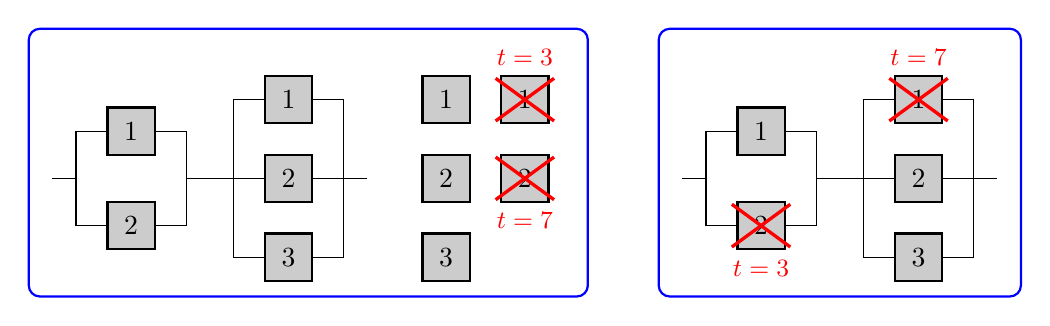
\begin{tikzpicture}
[type1/.style={rectangle,draw,fill=black!20,thick,inner sep=0pt,minimum size=6mm},
 type2/.style={rectangle,draw,fill=black!20,thick,inner sep=0pt,minimum size=6mm},
 type3/.style={rectangle,draw,fill=black!20,thick,inner sep=0pt,minimum size=6mm},
 cross/.style={cross out,draw=red,very thick,minimum width=7mm, minimum height=5mm},
 hv path/.style={to path={-| (\tikztotarget)}},
 vh path/.style={to path={|- (\tikztotarget)}}]
\node[type1] (double1) at ( 1, 0.6) {1};
\node[type2] (double2) at ( 1,-0.6) {2};
\node[type1] (triple1) at ( 3, 1)  {1};
\node[type2] (triple2) at ( 3, 0)  {2};
\node[type3] (triple3) at ( 3,-1)  {3};
\coordinate (start) at (0,0);
\coordinate (bifst) at (0.3,0);
\coordinate (bifen) at (1.7,0);
\coordinate (trist) at (2.3,0);
\coordinate (trien) at (3.7,0);
\coordinate (end)   at (4,0);
\path (start) edge (bifst)
      (bifst) edge[vh path] (double1.west)
              edge[vh path] (double2.west)
      (bifen) edge[vh path] (double1.east)
              edge[vh path] (double2.east)
              edge (trist)
      (trist) edge[vh path] (triple1.west)
              edge          (triple2.west)
              edge[vh path] (triple3.west)
      (trien) edge[vh path] (triple1.east)
              edge          (triple2.east)
              edge[vh path] (triple3.east)
              edge          (end);
%
\node[type1] at ( 5, 1) {1};
\node[type1, label={[red, font=\small]above:$t=3$}] %
             at ( 6, 1) {1};
\node[cross] at ( 6, 1) {};
\node[type2] at ( 5, 0) {2};
\node[type2, label={[red, font=\small]below:$t=7$}] %
             at ( 6, 0) {2};
\node[cross] at ( 6, 0) {};
\node[type3] at ( 5,-1) {3};
\draw [thick, rounded corners, blue] (-0.3,-1.5) rectangle (6.8,1.9);
%
\begin{scope}[xshift=8cm]
\node[type1] (double1) at ( 1, 0.6) {1};
\node[type2, label={[red, font=\small]below:$t=3$}] %
             (double2) at ( 1,-0.6) {2};
\node[cross] at ( 1,-0.6) {};
\node[type1, label={[red, font=\small]above:$t=7$}] %
             (triple1) at ( 3, 1)  {1};
\node[cross] at ( 3, 1) {};
\node[type2] (triple2) at ( 3, 0)  {2};
\node[type3] (triple3) at ( 3,-1)  {3};
\coordinate (start) at (0,0);
\coordinate (bifst) at (0.3,0);
\coordinate (bifen) at (1.7,0);
\coordinate (trist) at (2.3,0);
\coordinate (trien) at (3.7,0);
\coordinate (end)   at (4,0);
\path (start) edge (bifst)
      (bifst) edge[vh path] (double1.west)
              edge[vh path] (double2.west)
      (bifen) edge[vh path] (double1.east)
              edge[vh path] (double2.east)
              edge (trist)
      (trist) edge[vh path] (triple1.west)
              edge          (triple2.west)
              edge[vh path] (triple3.west)
      (trien) edge[vh path] (triple1.east)
              edge          (triple2.east)
              edge[vh path] (triple3.east)
              edge          (end);
%\node [draw, rounded corners,fit=(start) (double1) (double2) (triple1) (triple2) (triple3) (end)] {};
\draw [thick, rounded corners, blue] (-0.3,-1.5) rectangle (4.3,1.9);
\end{scope}
\end{tikzpicture}

\bigskip

Replacing in the notation for the prior parameter set $\PkZ = [\nkzl,\nkzu] \times [\ykzl,\ykzu]$
the $\yz$ component with the corresponding expected lifetime $(\ykz)^{1/\kappa} \Gamma(1 + 1/\kappa)$,
we assume $\PZi{1} = [2,5] \times [9, 11]$, $\PZi{2} = [4,8] \times [4, 6]$ and $\PZi{3} = [1,3] \times [9, 11]$,
and observe $\mbf{t}^1_{e_1;n_1} = (7, 7^+)$, $\mbf{t}^2_{e_2;n_2} = (3,7^+)$ and $\mbf{t}^3_{e_3;n_3} = (7^+)$,
so something that we more or less expect. Then the graph for $P(\Tsys > t\mid\PkZ, \mbf{t}^k_{e_k;n_k})$,
assuming we don't know which of the components of the same type have failed, is below:\\

\includegraphics[width=0.85\textwidth]{rsyspbox1}

This starts at $0.75$ as there is $1/4$ probability that the two failed components
are both in the first parallel part.

The grey shaded area is from optimization for each $t$ over the three $\nkz$ parameters,
while each of the black lines is from one the $8$ combinations of $\nkzfun{1}, \nkzfun{2}, \nkzfun{3}$
taking its lower or upper bound, for each $\ykzl$ and $\ykzu$, so $16$ combinations in total.

These $16$ combinations are depicted again below. It seems that for both $\ykzl$ (solid lines) and $\ykzu$ (dashed lines),
the combination "111" (lower $\nkz$ for all $k$) gives the lowest $\Rsys(t)$ for all $t$,
while combination "222" (upper $\nkz$ for all $k$) gives the highest $\Rsys(t)$ for all $t$,
but on close inspection we see that just after $t=10$, the green solid line goes below the
black solid line, so for larger $t$'s we get the lowest $\Rsys(t)$ for combination "121".
(It's difficult to see, but there is a hint of black above green around $t=11$.)
This might be due to the fact that we expect the mean component lifetime for components of type 2 to be lower than 6,
and are quite sure about that ($\nkz \in [4,8]$), so it seems very unlikely for the one remaining component of type 2
to survive past 10, triggering a situation of prior-data confict,
for which $\ykzl$ is obtained by $\nkzl$ instead of $\nkzu$.
So this unlikely situation is reflected in posterior inferences,
but the effect is small here because the survival of this system depends not only on the one remaining component of type 2,
but also of the two other remaing components.

\includegraphics[width=\textwidth]{fourKcornerSys1}

If we know instead which components have failed (see system graph, right),
then we must replace, in Equation~\eqref{eq:30}, the signature for the full system with the signature for the reduced system,
consisting of $n_1-e_1, \ldots, n_K-e_K$ components, so everything else in \eqref{eq:30} remains unchanged.
The graphs for this situation are below. There, we have again a switch from "111" to "121" at around $10.3$.

\includegraphics[width=0.5\textwidth]{rsyspbox1failed}
\includegraphics[width=0.5\textwidth]{fourKcornerSys1failed}


For this system and observed data, we have $l_k \in \{0,1\}$ for all $k$,
therefore $F(C_t^k)$ has only one step at $0$,
and so the problem of having different parameter pairs $(\nkz,\ykz)$ minimizing $F(C_t^k)$ for different $l_k$'s cannot appear.
This could also lead to a switch as above,
or even to the situation that a "non-corner" minimizes $\Rsys$ at a certain $t$.
Therfore, we consider the following system,
for simplicity consisting of only one type:\\

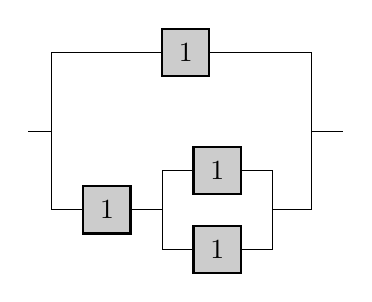
\begin{tikzpicture}
[type1/.style={rectangle,draw,fill=black!20,thick,inner sep=0pt,minimum size=6mm},
 type2/.style={rectangle,draw,fill=black!20,thick,inner sep=0pt,minimum size=6mm},
 type3/.style={rectangle,draw,fill=black!20,thick,inner sep=0pt,minimum size=6mm},
 cross/.style={cross out,draw=red,very thick,minimum width=7mm, minimum height=5mm},
 hv path/.style={to path={-| (\tikztotarget)}},
 vh path/.style={to path={|- (\tikztotarget)}}]
\node[type1] (upper)   at (2, 1) {1};
\node[type1] (lower)   at (1,-1) {1};
\node[type1] (double1) at (2.4,-0.5) {1};
\node[type1] (double2) at (2.4,-1.5) {1};
\coordinate (start) at (0,0);
\coordinate (bifst) at (0.3,0);
\coordinate (bifen) at (3.6,0);
\coordinate (end)   at (4,0);
\coordinate (doublest) at (1.7,-1);
\coordinate (doubleen) at (3.1,-1);
\path (start) edge (bifst)
      (bifst) edge[vh path] (upper.west)
              edge[vh path] (lower.west)
      (lower.east) edge[vh path] (doublest)
      (doublest)   edge[vh path] (double1.west)
                   edge[vh path] (double2.west)
      (doubleen)   edge[vh path] (double1.east)
                   edge[vh path] (double2.east)
      (bifen) edge (end)
              edge[vh path] (upper.east)
              edge[vh path] (doubleen);
\end{tikzpicture}

\bigskip

We assume $\PZi{1} = [2,5] \times [9, 11]$ and observe $\mbf{t}^1_{e_1;n_1} = (10, 11, 11^+, 11^+)$.
In the left graph below, for $t=12$ we have the standard situation that
$(\nkzl, \ykzl)$ ("bl", bottom left) delivers the lower cmf and 
$(\nkzu, \ykzu)$ ("tr", top right) delivers the upper cmf.
However, for $t=15$ and $t=20$, the upper resp.\ the lower cmf $F(C_t^k)$ depends on $\nkz$,
see the center and the right graph below.
(Difficult to see in the right graph, but I checked the numbers.)

\includegraphics[width=\textwidth]{cmfssys4}

This is then mirrored in $\Rsys(t)$, see graphs below, where the right one zooms in into the range $t \in [14,16]$.

\includegraphics[width=0.5\textwidth]{rsyspbox2}
\includegraphics[width=0.5\textwidth]{rsyspbox2zoom}

***have clear pdc situations in observed data already (so far only in posterior predictive scenario.)
\end{document}
